\chapter{Análisis del sistema} \label{cap:capitulo4}

Con este nuevo capítulo se da por terminado el proceso de ingeniería inversa al que se ha sometido a los limitadores \acrshort{LM7} y \acrshort{LM9}. De ellos se extrae una inmensa cantidad de información que nos será útil para diseñar y construir un sistema software que pueda correr bajo el nuevo prototipo de limitador disponible en el laboratorio ed \glsname{granasat}.

El software de los limitadores estudiados, aunque no presenta la mejor calidad, realiza su función, por lo que gran parte de éste será reutilizado en el nuevo sistema. Damos lugar por tanto a un proceso de análisis en el que se evaluará en qué grado los módulos de los \acrshort{LM7} y \acrshort{LM9} satisfacen las necesidades de nuestro sistema, así como las posibles mejores aplicables.

Por lo general, se prefiere el diseño y la implementación de la versión \acrshort{LM9} dado que está diseñado para funcionar sobre un hardware casi idéntico al del prototipo disponible: una Raspberry Pi. Esto desde luego no significa que la versión vaya a ser descartada; es importante recordar que ésta es la versión disponible físicamente en el laboratorio, y de la cuál se tiene certeza sobre su correcto funcionamiento. Además, recordemos que la versión \acrshort{LM9} supone una actualización, y no un software independiente. Por tanto, \textbf{siempre que surjan dudas} sobre el diseño o implementación de alguno de los módulos se irá sobre seguro y \textbf{se dará total preferencia a la versión \acrshort{LM7}}.

Tras el estudio de ambas versiones se hace evidente el hecho de que, al menos el código, no ha sido realizado de forma profesional, ya que hay problemas graves en el mismo. Algunos de ellos se listan a continuación:

\begin{enumerate} \label{sec:errores}
 \item No separar la declaración de las clases de su implementación (ficheros \texttt{.h} ó \texttt{.hpp} y \texttt{.cpp}, respectivamente).

 \item Inclusión directa de ficheros \texttt{.cpp}.

 \item Utilizar funciones y variables globales en lugar de clases.

 \item Violar completamente el \textit{Principio de Encapsulamiento}\footnote{En programación orientada a objetos, se denomina encapsulamiento al ocultamiento del estado, es decir, de los datos miembro de un objeto de manera que solo se pueda cambiar mediante las operaciones definidas para ese objeto} de la Programación Orientada a Objetos. Absolutamente todos los datos miembro de todas las clases tienen accesibilidad pública y son modificados directamente.

 \item Falta casi absoluta de un formato legible\footnote{Doy gracias al formateador de Visual Studio Code por preservar mi salud mental en éste sentido.} y de documentación.

 \item Nombre de variables poco descriptivos.

 \item Mal uso de la herramienta Makefile.

 \item Funcionalidades duplicadas.

 \item Excesiva complejidad en algunos programas (\commillas{MacGyver})\footnote{Término acuñado por un profesor de la ETSIIT, haciendo referencia a clases que \commillas{intentan hacerlo todo.}}.
\end{enumerate}

En la medida de los posible, se intentará solventar estos problemas en aquellos módulos que sean seleccionados para su integración en el proyecto, con el objetivo de dotar al código de un cierto grado \textbf{calidad} que facilite su lectura, comprensión y mantenimiento.

\section{Análisis hardware del prototipo}

En el laboratorio se dispone de un prototipo hardware sobre el que deberá ejecutarse el software a desarrollar, por tanto es necesario conocer sus componentes ya que pueden inyectar ciertas restricciones técnicas que deben ser tomadas en cuenta durante el proceso de diseño y desarrollo del producto.

\begin{itemize}

	\item En esencia, este equipo se basa en una \acrshort{PCB} o placa base hecha a medida sobre la que se conectan los distintos componentes.
	\item Como módulo de computación se tiene una Raspberry Pi modelo 3, sobre la que corre un sistema operativo \glsname{DietPi}, basada en una distribución de Linux.

	\item Para la entrada/salida de los canales de audio se dispone de 6 entradas balanceadas \acrshort{XLR}. Estas salidas pueden verse en la imagen \ref{img:lms11-xlr}. Por el momento el prototipo tan sólo dispone de un micrófono, aunque el objetivo es permitir la conexión de ambos en siguientes versiones del prototipo.

	\item El equipo dispone de un \acrshort{PGA} para llevar a cabo la atenuación. La diferencia entre por ejemplo, el \acrshort{LM7}, es que se dispone de un conmutador digital en lugar de un relé para realizar la redirección del audio hacia la salida.

	\item Como complementos, el prototipo dispone de una pequeña pantalla \acrshort{LCD} de 4 filas por 20 columnas; de un buzzer, y de una serie de \acrshort{LED}s RGB. Es deseable que el software pueda controlar estos componentes para poder mostrar mensajes haciendo uso de ellos.
\end{itemize}

\begin{figure}[h]
    \centering
    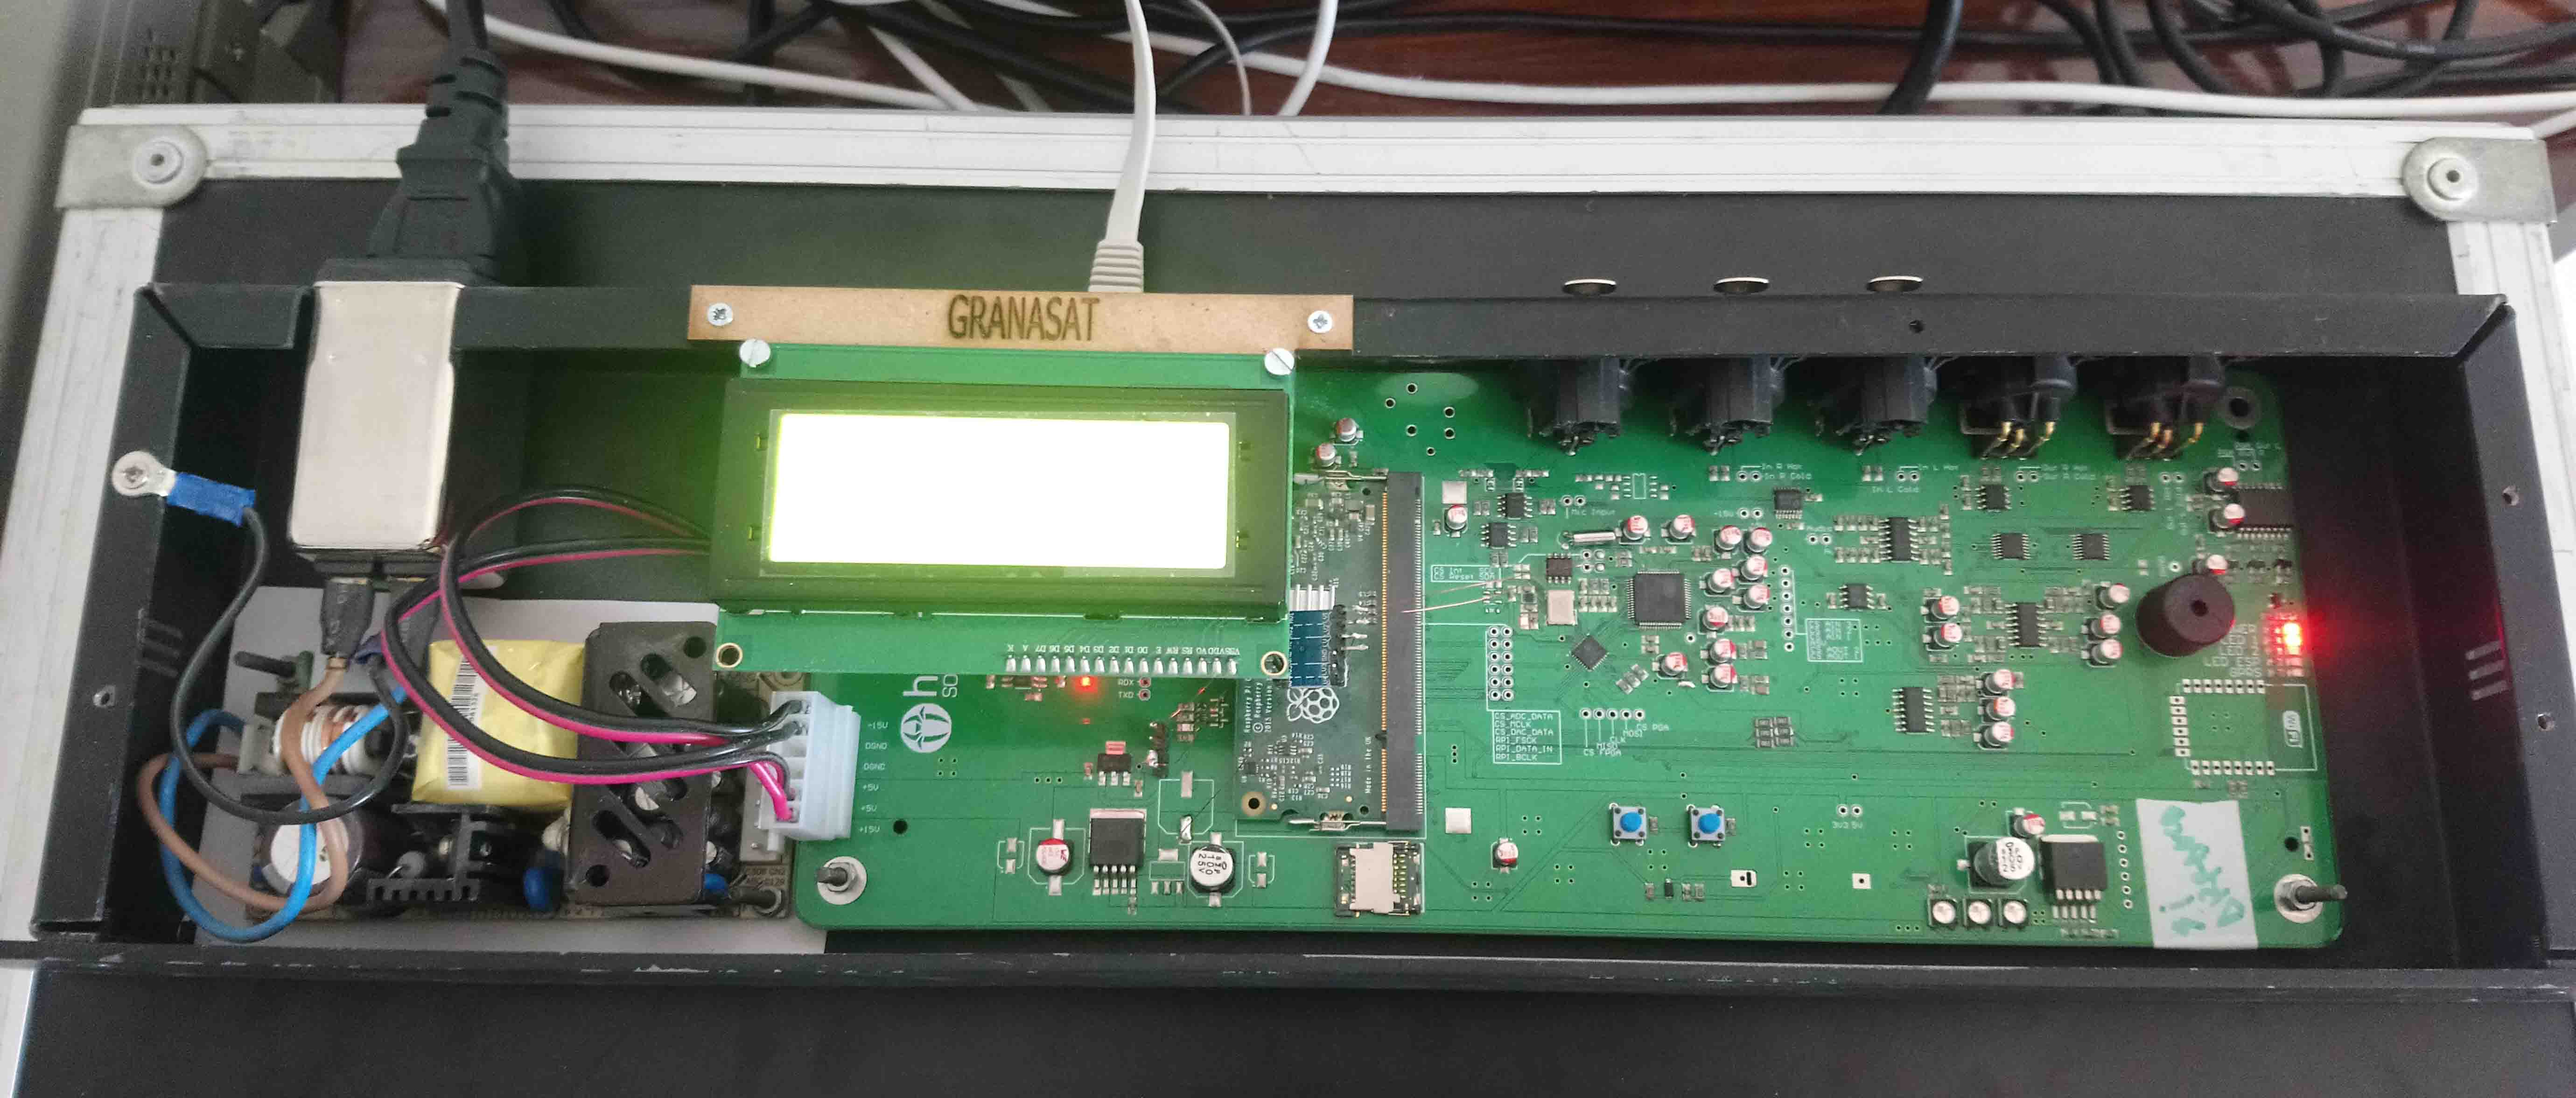
\includegraphics[width=0.9\textwidth]{imagenes/lm7-fotos/lms11.jpg}
    \caption{Uno de los modelos del prototipo de limitador disponible.}
    \label{img:lms11-hw}
\end{figure}

%\begin{enumerate}
%	\item IN: Micrófono #1.
%	\item IN: micrófono #2.
%	\item IN: canal izquierdo.
%	\item IN: canale derecho.
%	\item OUT: canal izquierdo.
%	\item OUT canal derecho
%\end{enumerate}

\subsection{Restricciones técnicas impuestas por el hardware}

Las especificaciones hardware del limitador impone una serie de restricciones técnicas a nuestro proyecto que debemos tener en cuenta. Las restricciones identificadas se transforman a requisitos no funcionales y se listan a continuación:

\begin{enumerate}
	\item Una Raspberry utiliza un microprocesador con arquitectura \textbf{\acrshort{ARM}}, por lo que debe tenerse a la hora de compilar el código C++.

	\item En este equipo disponemos de una única tarjeta de sonido personalizada, con 8 canales digitales.

	\item El interfaz de sonido a usar debe ser \acrshort{ALSA} (requisito impuesto por el cliente).

	\item Está planeado que el nuevo hardware admita dos micrófonos en un futuro, por lo que el software debe estar preparado para ello.
\end{enumerate}


\section{Evaluación de satisfacción requisitos}

A continuación se analizan los requisitos funcionales en base a lo aprendido en el proceso de ingeniería inversa. Para ello se estudia si el software estudiado permite satisfacer parte de los requisitos funcionales del proyecto, para así poder re-utilizarlos.

\begin{table}[h]
\centering
\begin{tabularx}{1\textwidth}{l|X}
Requisito  & RF 1.- Calibración de sensores                                                                 \\
Módulo     & LM9-calibrador                                                                              \\
Análisis   & Esta implementación y la del \acrshort{LM7} se basan en el mismo algoritmo, dónde funciona correctamente. \\
Evaluación & Válido
\end{tabularx}
\caption{Evaluación de satisfacción del RF-1}
%\label{tab:my-itable}
\end{table}

\begin{table}[h]
\centering
\begin{tabularx}{1\textwidth}{l|X}
Requisito  & RF 2.- Emisión de ruido rosa                                                                \\
Módulo     & LM7-script                                                                              \\
Análisis   & No aplicable debido al uso de dos tarjetas de sonido, mientras que nuestro prototipo sólo dispone de una. La idea subyacente, sin embargo, resulta útil al disponer el prototipo de un conmutador digital. \\
Evaluación & Re-utilizable
\end{tabularx}
\caption{Evaluación de satisfacción del RF-2}
%\label{tab:my-itable}
\end{table}

\begin{table}[h]
\centering
\begin{tabularx}{1\textwidth}{l|X}
Requisito  & RF 3.- Verificación                                                                \\
Módulo     & LM7-script                                                                             \\
Análisis   & El script, escrito en PHP, depende de funciones de la interfaz web. Habría que exportar estas dependenciase incluirlas en el propio script. \\
Evaluación & Válido
\end{tabularx}
\caption{Evaluación de satisfacción del RF-3}
%\label{tab:my-itable}
\end{table}

\begin{table}[h]
\centering
\begin{tabularx}{1\textwidth}{l|X}
Requisito  & RF 4.- Gestión de registro                                                                \\
Módulo     & Ambos-registrador                                                                           \\
Análisis   & Aunque en el \acrshort{LM9} el registrador se ha extraído a un programa independiente del limitador, el proceso de registro es el mismo. La manera en la que se almacenan los registros no es para nada la mejor, pero es la única que se tiene. Recrear el módulo (mediante por ejemplo una base de datos) supondría un gran riesgo para el proyecto debido al escaso tiempo del que se dispone. También supondría tener que rehacer por completo el módulo getData, ya que quedaría inservible. La mejora del sistema actual se deja como trabajo futuro. \\
Evaluación & Válido
\end{tabularx}
\caption{Evaluación de satisfacción del RF-4}
%\label{tab:my-itable}
\end{table}

\begin{table}[h]
\centering
\begin{tabularx}{1\textwidth}{l|X}
Requisito  & RF 5.- Interfaz de configuración y consulta                                                                 \\
Módulo     & LM7-Aplicación web                                                                           \\
Análisis   & La aplicación web está fuertemente acoplada al software del limitador y al sistema operativo. Por otra parte el código es bastante pobre, usa el obsoleto PHP 5 y depende de muchas librerías que a día de hoy también se encuentran obsoletas o directamente han desaparecido. Se ha intentado varias veces portar la interfaz por petición explícita del cliente pero sin éxito. En su lugar, \textbf{se propone una \glsname{API-REST}}. \\
Evaluación & Inviable
\end{tabularx}
\caption{Evaluación de satisfacción del RF-5}
%\label{tab:my-itable}
\end{table}

\begin{table}[h]
\centering
\begin{tabularx}{1\textwidth}{l|X}
Requisito  & RF 6.- Lectura de presión acústica                                                                 \\
Módulo     & LM9-analizador                                                                          \\
Análisis   & El analizador de audio del \acrshort{LM9} supone una importante mejora respecto a su versión anterior. Hace uso de \acrshort{ALSA}, lo que satisface uno de los requisitos no funcionales. Por otra parte, está diseñado para conectarse a un dispositivo de audio de \acrshort{ALSA}, lanzando 2 instancias de este programa, uno para cada tarjeta de sonido. Por una de ellas se obtiene el audio de las líneas y por la otra el audio de los micrófonos. Esto debe revisarse ya que en nuestro caso tan solo hay una tarjeta de sonido. El programa tendría por tanto que recuperar y analizar los datos de los 4 canales de entrada de forma simultánea, y el programa no está diseñado para leer de más de dos canales. \\
Evaluación & Re-utilizable
\end{tabularx}
\caption{Evaluación de satisfacción del RF-6}
%\label{tab:my-itable}
\end{table}

\begin{table}[h]
\centering
\begin{tabularx}{1\textwidth}{l|X}
Requisito  & RF 7.- Aplicación de atenuación                                                                \\
Módulo     & Ambos-limitador                                                                          \\
Análisis   & Los algoritmos en ambas versiones son completamente distintos. Se elige el proceso de atenuación del limitador \acrshort{LM7} como candidato. Sin embargo, debería someterse a un profundo proceso de refactoring ya que el resto de componentes software con los que se comunica se han tomado del \acrshort{LM9}, como el analizador de sonido o el registrador. La conexión con el nuevo hardware también debe rehacerse (detección de micrófono y comunicación con la \acrshort{PGA}). \\
Evaluación & Re-utilizable
\end{tabularx}
\caption{Evaluación de satisfacción del RF-7}
%\label{tab:my-itable}
\end{table}

\begin{table}[h]
\centering
\begin{tabularx}{1\textwidth}{l|X}
Requisito  & RF 8.- Discovery                                                               \\
Módulo     & Prototipo                                                                          \\
Análisis   & El equipo de \glsname{granasat} ya dispone de este mecanismo en versiones anteriores del prototipo. El mecanismo se basa en la emisión broadcast para llegar a todos los equipos en la misma red. \\
Evaluación & Válido
\end{tabularx}
\caption{Evaluación de satisfacción del RF-8}
%\label{tab:my-itable}
\end{table}

